\documentclass[11pt]{article}
\usepackage[margin=1in]{geometry}
\usepackage{amsmath,amssymb,amsthm}
\usepackage{booktabs}
\usepackage{enumitem}
\usepackage{graphicx}
\usepackage[T1]{fontenc}
\usepackage[hidelinks]{hyperref}
\usepackage{xcolor}
\usepackage{caption}
\captionsetup{font=small,labelfont=bf}
\setlist{nosep,leftmargin=1.4em}
\graphicspath{{../results/}}
\newcommand{\E}{\mathbb{E}}
\newcommand{\todo}[1]{\textcolor{red}{[#1]}}
\newcommand{\Fanon}{\mathcal{F}^{\mathrm{anon}}}
\newcommand{\Fid}{\mathcal{F}^{\mathrm{id}}}
\newcommand{\For}{\mathcal{F}^{\mathrm{oracle}}}

\title{\textbf{Rent or Toxicity? Strategic Exploitability of Learning Market Makers\\ with Public Wallet Information (Hyperliquid)}\\[0.4em]
\large Revised proposal and Workshop-1 report}
\author{Deepu Pradeep \quad Miguel Betran Menz \\
\normalsize 6.S974 Games, Learning, and Security --- Example 4 (Algorithmic Market with Adaptive Agents)}
\date{October 9, 2026 --- supersedes Deliverable 1 of October 6}

\begin{document}
\maketitle

\begin{abstract}
\noindent Independent reinforcement-learning market makers settle at spreads above the competitive level without communicating. A wide spread is either \emph{rent} that an entrant can capture or the correct price of \emph{toxic} order flow, and the two look identical on the tape. We study the entrant's problem on Hyperliquid, an on-chain order book where every print carries both counterparties' wallet addresses. This document revises our October~6 proposal in light of three days of simulation and the first Hyperliquid data. Three things changed. (1)~The exploitability hypothesis ``more collusive $\Rightarrow$ more exploitable'' holds only in a trivial form; the fraction of rent a profit-maximising entrant destroys is flat at $\approx 0.7$ across populations, so RQ2 is restated as a measurement. (2)~The mechanism by which wallet identity pays is not wallet persistence (same-wallet repeats are $3$--$4\times$ chance but only $0.02$--$0.05$ in level); it is that informed flow clusters in time and a toxic wallet's print reveals the regime \emph{before the price does}. The simulator now has a latent toxicity regime and a lag between a print and its mark, and with them identity's value reappears where the data say it should. (3)~The quoted spread on BTC, ETH and SOL is pinned at one tick essentially all the time, so on those books rent cannot live in the spread; it can only live in which fills a maker gets. We lay out the revised model, the results that forced the revisions, the calibration numbers, and the plan to a December preprint.
\end{abstract}

\section{Motivation and central claim}
Market makers (MMs) post bids and asks, earn the spread from impatient traders, and lose to \emph{informed} traders whose orders predict the next price move. Increasingly they are learning algorithms. Three facts make this a trading-firm problem rather than only a regulator's. (i)~Independent learning MMs drift to spreads above the competitive level without communicating \cite{contxiong,cfl}. (ii)~A spread above competitive is rent an entrant can capture by undercutting, but the same wide spread is also the correct response to toxic flow: identical observable, opposite action. (iii)~Optiver reports that current LLM traders name adverse selection yet trade at negative expected value and fail to model how others react \cite{optiver}. The skill a desk wants---read the tape, decide whether competitors are soft or the flow is poisonous, and quote accordingly without becoming the exploited party---has no quantitative benchmark.

\paragraph{Central claim, revised.} Learning market makers earn supra-competitive rents that survive entry: a simple entrant that reads markouts off the public tape takes most of the rent and keeps it when the incumbents are allowed to re-learn, because the cartel re-forms around the entrant rather than collapsing. The entrant's problem is therefore not whether rent exists but \emph{which flow to take}, and that is a regime-inference problem. On a venue with public wallet identity, the identity of the last taker reveals the toxicity regime before the price move that would reveal it anonymously; the lag between a print and its mark is where the value of identity lives. On tick-constrained books, where the spread cannot widen, the same fill-selection mechanism is the only place rent can live at all.

The pieces exist separately: learned rents \cite{cfl,contxiong}; strategic exploitation of learners in abstract games \cite{dss,brownmackay}; on Hyperliquid, persistent wallet histories carry adverse-selection information \cite{zhai} and disclosed flow changes impact \cite{barone}. What is new here is the chain: learned rent $\to$ entrant best response $\to$ value of public identity, measured in the same units in the simulator and on the venue.

\section{What changed since Deliverable 1, and why}\label{sec:changes}
Table~\ref{tab:changes} is the audit trail. Every row is a claim in the October~6 text, the finding that bears on it, and the change made. Code, results and a running findings log are at \url{https://github.com/pradeepu191/wargame} (\texttt{results/REPLICATION\_NOTES.md}).

\begin{table}[h]\small\centering
\begin{tabular}{p{0.3\textwidth}p{0.36\textwidth}p{0.28\textwidth}}
\toprule
\textbf{Deliverable 1 said} & \textbf{What we found} & \textbf{Change} \\
\midrule
RQ2 hypothesis $\partial L_{\mathrm{BR}}/\partial C>0$: the regularity that sustains rents makes policies easier to manipulate. & Slope of $L_{\mathrm{BR}}$ on $C$ is $\approx1$ by construction (more rent, more to lose); the \emph{fraction} of rent destroyed is flat at $\approx0.7$ (\S\ref{sec:exploit}). & Restated as a measurement; attacker set split into damage-maximising and profit-maximising. \\
\addlinespace
Identity matters because wallet toxicity is a persistent trait (Zhai's ten-day persistence). & Same-wallet repeat rate at the order level is $0.02$--$0.05$; identity's effect on the next fill's markout is $0.5$--$0.9$ bps and survives conditioning on the anonymous tape (\S\ref{sec:data}). & Simulator: latent toxicity regime + mark lag replace wallet persistence (\S\ref{sec:takers}); RQ1 restated. \\
\addlinespace
Rent appears as a quoted spread above break-even; undercutting means quoting tighter. & Quoted spread on BTC/ETH/SOL is one tick, p90 $=$ median, over six hours of book data (\S\ref{sec:l2}). & Spread game kept as theory and for books that open beyond a tick; on tick-bound books rent is reinterpreted as fill selection; queue model added to plan. \\
\addlinespace
Markouts from the trade tape. & Trade-price proxy carries bid--ask bounce; true-mid adverse selection is $-0.33$ bps on all four coins. & L2 recorded; all markouts now against the true mid. \\
\addlinespace
MM wallets avoid each other (CCG signature). & Avoidance ratio $\approx1$ on 374 classified wallets; below 1 only among the top-10 on thin books; unstable across windows. & Not claimed until a fixed wallet set over a longer window exists. \\
\addlinespace
Entrant quote rule: undercut when rent $\ge 2$ ticks. & A margin makes a \emph{better-informed} entrant earn less (it declines positive-EV fills when pessimistic). & Break-even rule (margin 1); first identity grid flagged for re-run. \\
\bottomrule
\end{tabular}
\caption{Audit of claims in Deliverable 1 against findings to date.}\label{tab:changes}
\end{table}

\section{Model}\label{sec:model}

\subsection{Market}
One contract, discrete time $t=1,\dots,T$ (one block per period, $T=100$ per episode), $N$ quoting MMs on a tick grid of size $\theta$. Each MM $i$ posts symmetric quotes at half-spread $h^i_t\in\{1,\dots,K\}$ ticks around the mid $m_t$. One taker arrives per period: informed with probability $\alpha$, else a liquidity trader with private valuation $m_t+L$, $L\sim N(0,\sigma_L^2)$, who buys if the best ask is below her valuation and sells if the best bid is above it. The fundamental is $V_t = m_t \pm d$, $d\sim\mathrm{Exp}(\mu)$, redrawn each period; an informed taker trades only when $d$ exceeds the best half-spread, so no quote is immune and, by memorylessness, an informed fill costs the maker exactly $\mu$ in expectation at every spread. (Deliverable~1's binary-$V$ specification had an adverse-selection cliff---any half-spread beyond the edge was immune---which tabular learners find and sit on; the exponential edge removes it while keeping closed forms.) The taker hits the best quote; ties split uniformly; the maker's profit per fill is $(p-V_t)$ on a sale, $(V_t-p)$ on a purchase.

\paragraph{Benchmarks (closed form).} With $x=h\theta$, the market-wide expected one-period profit of quoting $h$ is
\[
\Pi(h;\alpha)=(1-\alpha)\,2x\,\bar\Phi(x/\sigma_L)\;-\;\alpha\,\mu\,e^{-x/\mu},
\]
linear in $\alpha$. The competitive half-spread $h^C$ is the first grid point with $\Pi\ge0$ (Bertrand undercutting stops there), the joint-monopoly $h^M$ maximises $\Pi$, and $\Pi^C,\Pi^M$ are the profits at those points. The collusion index of a population is $\Delta=(\bar\Pi-\Pi^C)/(\Pi^M-\Pi^C)$ \cite{calvano}; we write $C(\pi)$ for the same quantity when the population is frozen and evaluated. With $\theta=0.5$, $K=24$, $\sigma_L=8$, $\mu=5$: $(h^C,h^M)=(2,13)$ at $\alpha=0.1$, $(4,14)$ at $0.3$, $(8,17)$ at $0.5$; $\Pi^M-\Pi^C$ falls from $1.90$ to $0.66$, so less rent is available where flow is more toxic.

\subsection{Takers with identity: types, regime, and the mark lag}\label{sec:takers}
This subsection replaces the ``persistent wallet id'' sentence of Deliverable~1 and is the main modelling change.

\paragraph{Types.} A population of $M$ wallets ($M=50$) with persistent types $\alpha_j$, taken as stratified quantiles of $\mathrm{Beta}(\bar\alpha\kappa,(1-\bar\alpha)\kappa)$ so that the mean is pinned at $\bar\alpha$ and the concentration $\kappa$ sets only the dispersion ($\kappa\to\infty$ recovers the homogeneous model). Wallet $j$'s order is informed with probability $\alpha_j$.

\paragraph{Regime.} A latent state $z_t\in\{\text{calm},\text{toxic}\}$, kept with probability $\rho_z$ and otherwise redrawn from a stationary law chosen so the stationary mean toxicity equals $\bar\alpha$. Wallet activity depends on the state: in the toxic state arrival weights are $\propto w_j\alpha_j$, in the calm state $\propto w_j(1-\alpha_j)$. With $\kappa=1$ the two states have toxicity $0.15$ and $0.65$ around $\bar\alpha=0.3$. The identity of the last print is therefore evidence about the regime the \emph{next} arrival shares, whoever it is. (A separate same-wallet persistence parameter $\rho$ remains in the code; the data put it near zero and it is off in all results below.)

\paragraph{Public information and the mark lag.} After commitment, a print is public: event, price, and wallet id. Its \emph{mark}---the ex-post value $V_t$ against which the fill's profit is measured---becomes public $L$ periods later (\texttt{mark\_lag}). Deliverable~1 implicitly had $L=1$, which gives an anonymous observer oracle-quality markouts before the next arrival. On Hyperliquid the next order arrives in $0.4$--$1.8$\,s and markouts realise over seconds to minutes; $L$ is the number of arrivals that elapse before the tape reveals what identity revealed at the print. Information sets are nested:
\[
\Fanon_t \subset \Fid_t \subset \For_t ,
\]
no ids / committed wallet ids / the true types. Nobody ever sees the identity of the order about to hit them.

\subsection{Agents}
\paragraph{Incumbents.} Tabular Q-learning \cite{calvano,cfl}: state $=$ (own last half-spread, min rival last half-spread), action $=$ half-spread, $\varepsilon$-greedy with $\varepsilon_t=e^{-\beta t}$, learning rate $\eta$, discount $0.95$, $2\times10^4$ episodes. Incumbents are identity-blind by construction, so the identity experiments measure what identity is worth to a newcomer against an identity-blind cartel. ``Re-learning'' incumbents resume Q-learning after entry with a fresh exploration schedule.

\paragraph{Entrants.} All see only public information.
\begin{itemize}
\item \emph{Competitive-GM}: quotes $h^C(\bar\alpha)$, ignores everyone. The textbook benchmark.
\item \emph{One-tick undercut}: one tick inside the best incumbent quote. The myopic upper bound if nobody punishes.
\item \emph{Own-fill markout} (Deliverable~1's ``markout rule''): estimates toxicity from the sign of its own fills' profits and undercuts when the implied rent is positive.
\item \emph{Wallet entrant} under $\Fanon$, $\Fid$ or $\For$: exact grid-Bayes estimation of $\bar\alpha$ from every period (print or not, since the best quote is public) and of each wallet's $\alpha_j$ from its prints with a print-conditional likelihood (no fill-selection bias; after 300 episodes the population estimate is within $0.005$ of truth and per-wallet error $0.03$). A two-state filter tracks $b_t=P(z_t=\text{toxic})$: with ids the evidence at a print is \emph{who} printed (likelihood ratio $\alpha_j(1-\bar\alpha)/((1-\alpha_j)\bar\alpha)$); without ids the evidence at the print is only that a print occurred, and the sign of its profit arrives $L$ periods later and is carried to the present through $\rho_z^{L}$ (the keep-or-redraw chain is reversible, so this is exact). Forecast $\alpha_{\mathrm{next}}=b\,\alpha(\text{toxic})+(1-b)\,\alpha(\text{calm})$. Quote rule: with best incumbent quote $b^*$, undercut to $\min(b^*-1,\,h^M(\alpha_{\mathrm{next}}))$ when $b^*-1\ge h^C(\alpha_{\mathrm{next}})$, else quote $h^C(\alpha_{\mathrm{next}})$, which for a toxic forecast is wider than the incumbents and amounts to withdrawing.
\end{itemize}

\subsection{Statistics}
\begin{itemize}
\item $\Delta$ / $C(\pi)$ as above; a \emph{mechanism test}: in states where a rival quotes at or inside the monopoly point, is the learner's greedy action its myopic best response (undercut) or restraint? Restraint share, forgone one-period reward, and Q-gap are reported.
\item Exploitability: $\Pi_{\mathrm{nominal}}$ (frozen incumbents alone), $J(\pi;A)$ (incumbents' profit with attacker $A$), $L^A_{\mathrm{BR}}=\Pi_{\mathrm{nominal}}-J$, $L_{\mathrm{BR}}=\max_A L^A_{\mathrm{BR}}$, and $\kappa_A=L^A_{\mathrm{BR}}/(\Pi_{\mathrm{nominal}}-\Pi^C)$, the fraction of rent destroyed. Entrant profit is reported in rent units $(\Pi^M-\Pi^C)$ so $N$ and $\alpha$ are comparable.
\item Value of information: $\pi^{\mathrm{id}}-\pi^{\mathrm{anon}}$ and $\pi^{\mathrm{oracle}}-\pi^{\mathrm{id}}$, paired by seed and market realisation (common random numbers).
\item Adverse-selection shift: informed share of the entrant's fills vs the incumbents' fills vs the market without the entrant.
\end{itemize}

\subsection{What is deliberately simple, and what the data say about it}
Unit size, symmetric quotes, risk-neutral makers, exogenous taker mix, no inventory in the state (inventory buckets are implemented and off), no fees or rebates, no request budgets, no liquidation flow. Two of these are now known to matter on the venue. The spread on the major books is one tick (\S\ref{sec:l2}), so the symmetric-half-spread action does not describe BTC/ETH/SOL under normal conditions; it describes thin books (HYPE opens to two ticks) and stress. And the archive records each counterparty's pre-trade position on every print, so inventory paths of real MM wallets are observable and the inventory-skew benchmark can be calibrated rather than assumed.

\section{Hyperliquid: mechanics and data}\label{sec:hl}
\paragraph{Mechanics as treatment arms} (unchanged from Deliverable~1 except where noted). Persistent pseudonymous wallet addresses on every committed order and both sides of every print. Per-user request budgets earned by filling, so the only ``drain'' attack is \emph{induced self-exhaustion} of a reactive rival. A priority fee that buys $\approx45$\,ms/bp for aggressive orders and queue position for resting ones \cite{hldocs}. A price grid of at most five significant figures: at current prices one tick is \$1 on BTC, \$0.10 on ETH, \$0.01 on SOL, \$0.001 on HYPE, i.e.\ $0.12$, $0.39$, $0.87$ and $0.11$\,bps respectively---and \S\ref{sec:l2} shows the spread sits on it. A protocol vault (HLP) with undisclosed strategies, which we treat as a calibration target for a fixed-policy benchmark, not a known policy. Liquidation flow routed to the book, with the October~10, 2025 cascade as the stress case.

\paragraph{Archive.} Albers et al.\ \cite{albers}, Zenodo record 18184441: trades for all perpetuals October 2025--January 2026 (JSON lines, both counterparties with pre-trade position, order ids, TWAP flags); order lifecycles and book diffs for BTC/ETH/SOL in December 2025. Two facts not in the schema document that matter for use: \texttt{side\_info} is $[\text{buyer},\text{seller}]$ (verified on 3.4M trades by the order-id rule: the aggressor's order is the newer one in 97.1\% of trades; the other 2.9\% are aggressors \emph{older} than the resting order, which is what triggered stop and liquidation orders look like, and are flagged); and the L1 hash is all zeros for orders filled in their submission block, so it cannot be an order key---fills of one sweep are collapsed on (block time, taker, side). January coverage is Jan 1--3 and Jan 19--31; we used Jan 26--28 (72\,h, 3.42M prints on BTC/ETH/SOL/HYPE, 1.44M taker orders).

\paragraph{Live feed.} A recorder on the public WebSocket (\texttt{data/record.py}) writes trades with both wallets, L2 snapshots, and the top of book on every change. 24\,h of trades (Oct 6--7, 871k prints) and 6\,h with the book (Oct 8). The feed and the archive agree on every structural statistic (\S\ref{sec:data}).

\paragraph{Pipeline.} \texttt{analysis/calibrate.py} turns either source into one row per coin: activity, markouts (proxy and true-mid), same-taker repeat rate at the order level against its random-matching baseline, split-half rank correlation of per-taker markouts, the conditional markout after a toxic vs a benign wallet's order, the same split conditioned on the anonymous ``price already moved against the last maker'' signal, MM wallet classification with a shuffled-label null for turn-taking, and the book statistics. Classification always uses the first half of a sample and measurement the second.

\section{Results to date}\label{sec:results}
All simulator results: $\theta=0.5$, $K=24$, $\sigma_L=8$, $\mu=5$, common random numbers across policies within a cell, means over seeds with seed-level standard deviations where quoted.

\subsection{Replication of learned supra-competitive spreads}
Two or three Q-learners ($\eta=0.15$, $\beta=4\times10^{-6}$, 10 seeds) settle at half-spreads of 10.6, 14.4 and 17.4 ticks for $\alpha=0.1,0.3,0.5$ against competitive 2, 4, 8 and monopoly 13, 14, 17: $\Delta=0.83$, $0.86$, $0.77$ (seed sd $0.01$--$0.02$). A robustness grid at $\alpha=0.3$ over $N\in\{2,3,5\}$, $\eta\in\{0.05,0.15\}$ and optimistic/pessimistic initialisation gives $\Delta=0.71$--$0.87$ in every cell (Table~\ref{tab:robust}); the slow learners ($\eta=0.05$) quote tighter. The mechanism test says this is restraint, not under-exploration: in 55--83\% of visited states a rival sits at or inside the monopoly quote, and in 96--100\% of those the learner's greedy action forgoes the myopic undercut. The best-quoter identity switches between episodes 45--70\% of the time: a turn-taking convention, not a fixed leader.

\begin{table}[h]\small\centering
\begin{tabular}{ccccccc}
\toprule
$N$ & $\eta$ & init & half-spread & $\Delta$ & restraint $\mid$ contested & leader switch \\
\midrule
2 & 0.05 & 0 & 11.2 & 0.84 & 1.00 & 0.52 \\
2 & 0.15 & 0 & 14.4 & 0.86 & 0.99 & 0.45 \\
3 & 0.05 & 0 & 9.3 & 0.72 & 0.98 & 0.61 \\
3 & 0.15 & 0 & 14.9 & 0.86 & 0.99 & 0.58 \\
5 & 0.05 & 0 & 9.7 & 0.71 & 0.97 & 0.63 \\
5 & 0.15 & 0 & 15.0 & 0.87 & 0.99 & 0.62 \\
\bottomrule
\end{tabular}
\caption{Robustness grid at $\alpha=0.3$ (10 seeds; optimistic-initialisation rows omitted, within $0.03$ of these). $h^C=4$, $h^M=14$.}\label{tab:robust}
\end{table}

\subsection{Does rent create vulnerability? (RQ2)}\label{sec:exploit}
120 frozen populations (the robustness grid plus the main runs at three $\alpha$; $C$ from $0.43$ to $0.97$ at the seed level) each face four attackers for 500 episodes. Figure~\ref{fig:exploit} and Table~\ref{tab:exploit}.

\begin{figure}[h]\centering
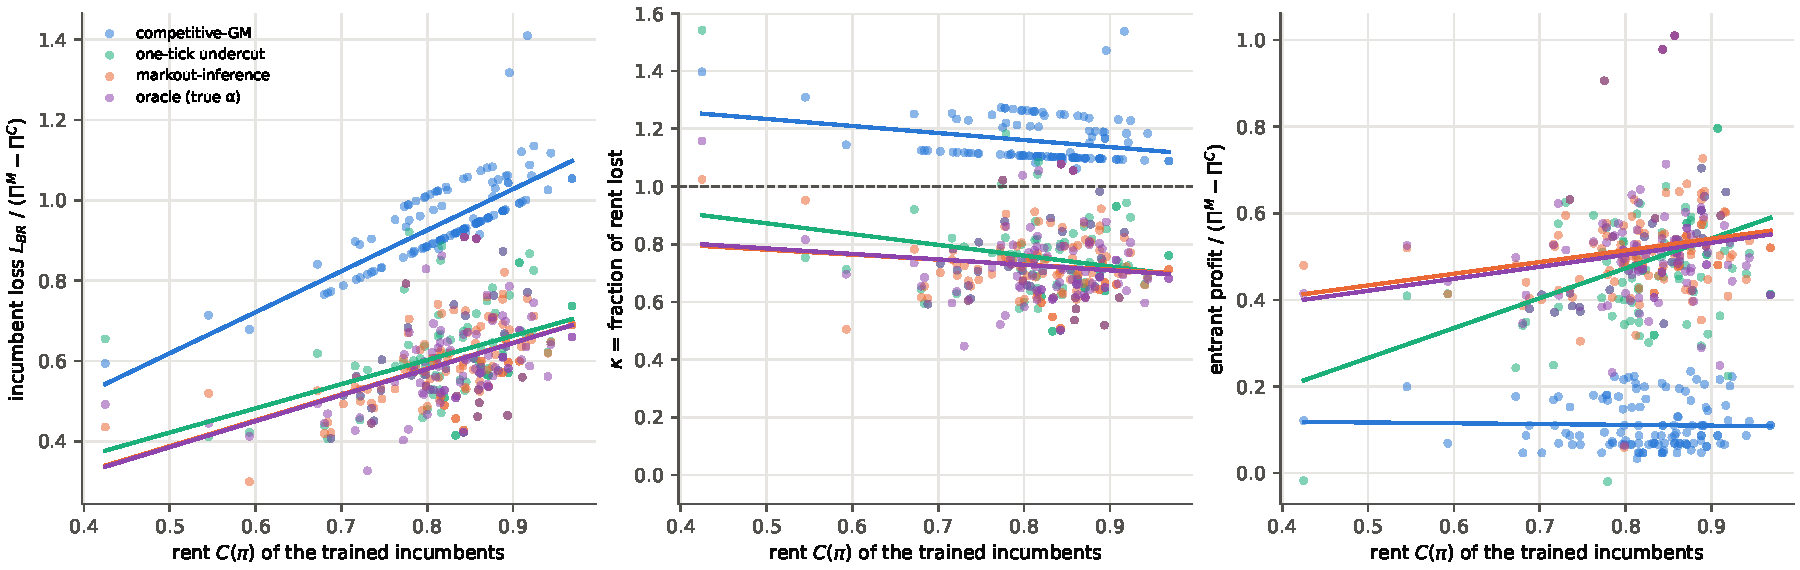
\includegraphics[width=\textwidth]{fig_exploitability.pdf}
\caption{Best-response loss, fraction of rent destroyed, and attacker profit against the incumbents' rent $C(\pi)$, 120 populations, one point per population and attacker.}\label{fig:exploit}
\end{figure}

\begin{table}[h]\small\centering
\begin{tabular}{lccc}
\toprule
slope on $C$ (OLS, bootstrap 95\% CI) & pooled & $\alpha=0.3$ only & within cell (seeds) \\
\midrule
$L_{\mathrm{BR}}$, max over attackers & $0.99\ [0.85,1.19]$ & $1.04\ [1.00,1.09]$ & $1.06\ [0.93,1.27]$ \\
$L_{\mathrm{BR}}$, markout attacker & $0.64\ [0.47,0.87]$ & $0.89\ [0.68,1.09]$ & $0.63\ [0.48,0.88]$ \\
$\kappa$, markout attacker & $-0.17\ [-0.46,0.23]$ & $0.27\ [-0.01,0.54]$ & $-0.24\ [-0.49,0.17]$ \\
$\kappa$, undercut attacker & $-0.37\ [-0.97,0.26]$ & $0.25\ [-0.02,0.54]$ & $-0.53\ [-1.21,0.29]$ \\
entrant profit, markout attacker & $0.27\ [0.10,0.50]$ & $0.61\ [0.37,0.94]$ & $0.10\ [-0.10,0.29]$ \\
\bottomrule
\end{tabular}
\caption{Regressions on rent across 120 frozen populations. $\kappa$ is the fraction of rent destroyed.}\label{tab:exploit}
\end{table}

\begin{itemize}
\item The literal hypothesis holds, by construction. The attacker that minimises incumbent profit is the competitive-GM quoter in 119 of 120 populations, and it pushes the incumbents \emph{below} $\Pi^C$ (frozen incumbents sometimes respond to a quote at $h^C$ by undercutting it and lose), so $L_{\mathrm{BR}}\approx\Pi_{\mathrm{nominal}}$ and the slope is one.
\item The substantive version is not supported. $\kappa$, the fraction of rent a profit-maximising attacker destroys, is $\approx0.7$--$0.8$ for undercut, markout and oracle attackers across the whole range of $C$, with slopes whose intervals include zero. Higher-rent populations are exploitable in proportion to their rent, not more.
\item Damage and profit are different objectives. The attacker that hurts the incumbents most earns least ($0.08$ rent units); the ones that earn most (markout, oracle: $0.50$) leave the incumbents 30\% of their rent. The markout rule is the attacker's own best response in 68 of 120 populations, the oracle in 36, the undercutter in 16.
\item Knowing the true $\alpha$ adds nothing over estimating it from own fills ($0.50$ vs $0.51$). In a stationary market the public tape carries the full value of the toxicity \emph{level}. This is the observation that sent us to heterogeneous takers.
\end{itemize}

\subsection{Entry: frozen and re-learning incumbents (RQ1, first form)}
Against frozen two-maker cartels, the own-fill markout entrant captures 79\%, 96\% and 93\% of the monopoly rent at $\alpha=0.1,0.3,0.5$ (entrant profit $0.95$, $0.72$, $0.36$ per period); the one-tick undercutter 84\%, 89\%, 75\%; the competitive quoter 18\%, 8\%, 14\%. The entrant wins 54--62\% of fills, not all of them: it wins the fills at profitable prices.

With incumbents that resume learning ($\varepsilon_0=0.3$ decaying to $0$ over 8000 episodes, Figure~\ref{fig:relearn}), the three policies produce three outcomes. The competitive entrant collapses the cartel: market $\Delta\to0$, the best quote sits at $h^C$, the entrant wins every fill and earns exactly $\Pi(h^C)$, and the re-learning incumbents converge to zero profit. The undercut and markout entrants let the cartel \emph{re-form around them}: $\Delta$ rises as exploration decays ($0.28\to0.62$ at $\alpha=0.5$ for markout), the best quote drifts wider, and the entrant's final profit equals its frozen-incumbent profit ($0.95/0.67/0.39$ vs $0.95/0.72/0.36$). Collapsing the cartel is the worst thing an entrant can do to itself: quoting at $h^C$ leaves 59\%, 82\% and 72\% of the markout entrant's profit on the table. Inference beats blind undercutting at every $\alpha$ and every stage, most during exploration ($\alpha=0.5$, first window: $0.25$ vs $0.03$), because the undercutter follows exploring incumbents into loss-making quotes.

\begin{figure}[h]\centering
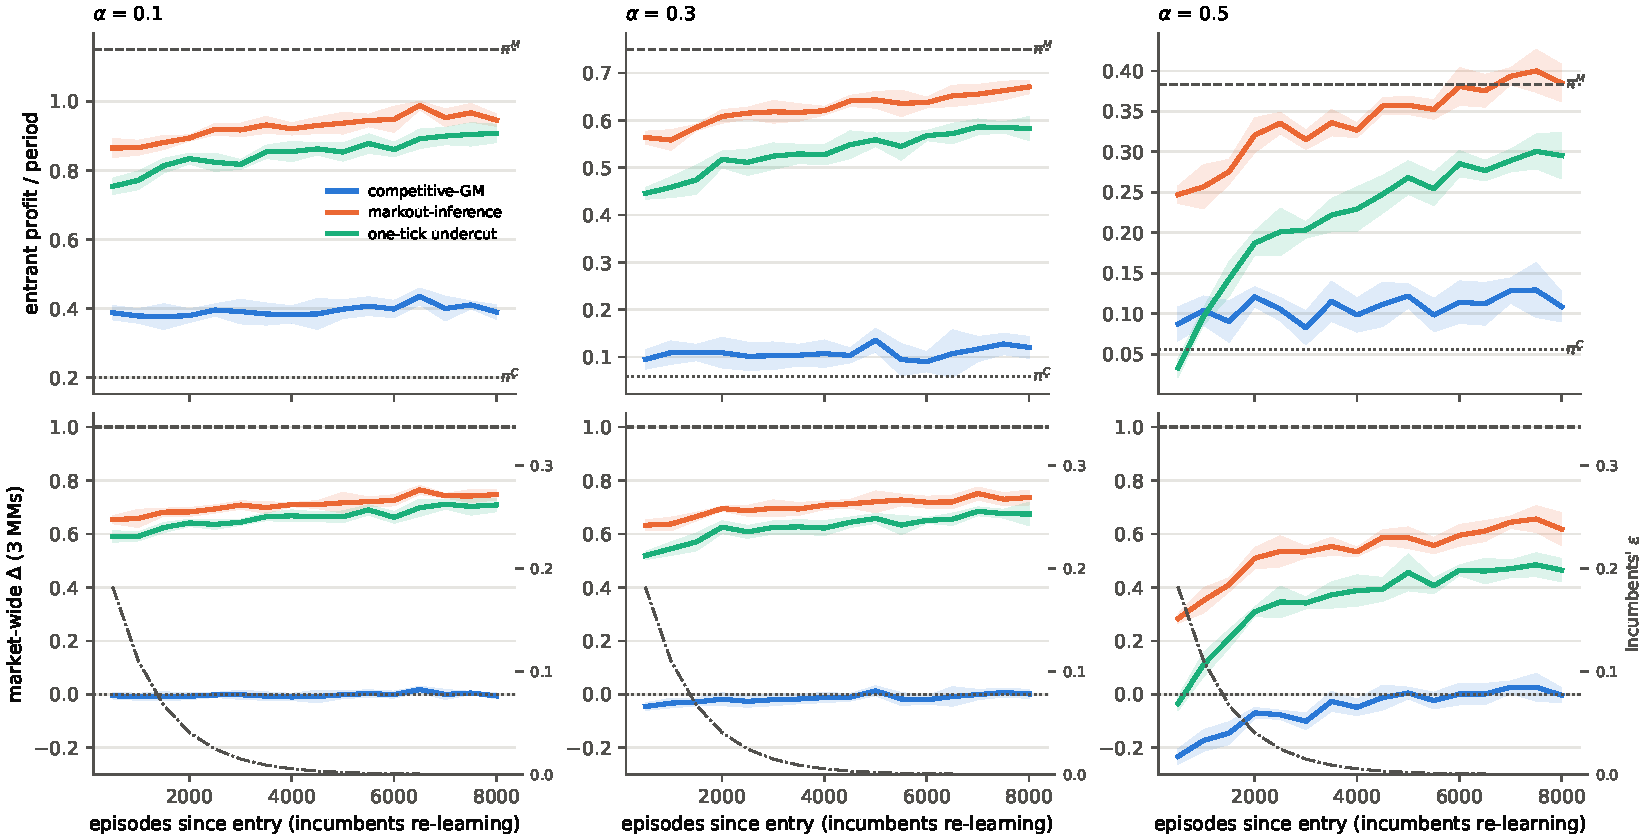
\includegraphics[width=\textwidth]{fig_cfl_exp2_entry_relearn.pdf}
\caption{Entry against re-learning incumbents: entrant profit (top) and market-wide $\Delta$ (bottom) over 8000 episodes, incumbents' $\varepsilon$ on the twin axis. Dashed/dotted lines are per-incumbent $\Pi^M$, $\Pi^C$ of the pre-entry market.}\label{fig:relearn}
\end{figure}

\subsection{The value of identity in the simulator (RQ1, revised form)}\label{sec:identity}
Three grids against frozen two-maker cartels, five seeds, entrant profit in rent units.

\paragraph{(a) Wallet persistence (the Deliverable-1 mechanism).} With same-wallet persistence $\rho$ and dispersion $\kappa$, identity is worth nothing at $\rho=0$ or $\kappa=\infty$ and $+0.16$ to $+0.30$ rent units (26--35\% of entrant profit) at $\rho=0.9$--$0.99$, $\kappa=1$; the identity entrant attains the oracle. The mechanism is fill selection: at $\bar\alpha=0.5$, $\rho=0.99$ it withdraws in 31\% of periods, its fills are 18\% informed against the incumbents' 53\%, and the identity-blind cartel's residual book goes below $\Pi^C$ while market $\Delta$ stays at $0.9$---the rent moved to the entrant (Figure~\ref{fig:as}). This grid used the margin-2 quote rule and is flagged for re-run; the qualitative result does not depend on it.

\begin{figure}[h]\centering
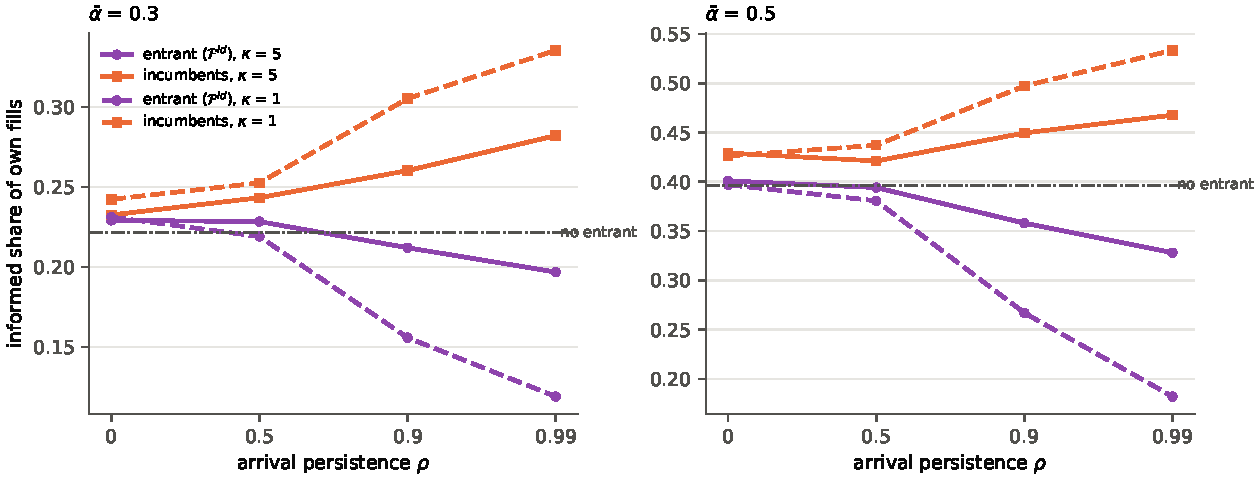
\includegraphics[width=0.85\textwidth]{fig_cfl_exp2_identity_as.pdf}
\caption{Adverse-selection shift under wallet persistence: informed share of the identity entrant's fills vs the incumbents', by persistence $\rho$ and dispersion $\kappa$.}\label{fig:as}
\end{figure}

\paragraph{(b) Regime, mark revealed immediately ($L=1$).} Replacing wallet persistence by the regime (\S\ref{sec:takers}) with $\rho=0$, identity's increment falls to $+0.01$ to $+0.08$: the anonymous tape already carries the regime because the last print's \emph{outcome} is as good a regime signal as its author. Identity pays only where the toxic state crosses the entrant's decision threshold (at $\kappa=1$, $\bar\alpha=0.5$: oracle $+0.15$).

\paragraph{(c) Regime with the mark lag.} Table~\ref{tab:lag}. At $\bar\alpha=0.5$ the anonymous entrant's profit falls as the mark arrives later ($0.97\to0.89$ at $\rho_z=0.99$) while the identity entrant's is flat, so identity's increment grows from $+0.05$ to $+0.13$ (every seed positive at $\rho_z=0.9$, $L=20$). At $\bar\alpha=0.3$ the lag changes nothing, because against $\sim11$-tick incumbents even the toxic state leaves an undercut profitable and the regime is not decision-relevant. The value of the wallet tag to an inside quoter is largest where the resting spread is close to the toxic-regime break-even. That is a prediction about \emph{which} books reward identity-aware quoting.

\begin{table}[h]\small\centering
\begin{tabular}{llccccc}
\toprule
$\bar\alpha$ & $\rho_z$ & $L$ & anon & id & oracle & id $-$ anon (paired) \\
\midrule
0.3 & 0.9 & 1 / 5 / 20 & 0.65 / 0.65 / 0.65 & 0.68 / 0.67 / 0.68 & 0.69 & $+0.03$ / $+0.03$ / $+0.03$ \\
0.3 & 0.99 & 1 / 5 / 20 & 0.78 / 0.80 / 0.79 & 0.80 / 0.81 / 0.80 & 0.84 & $+0.02$ / $+0.02$ / $+0.01$ \\
0.5 & 0.9 & 1 / 5 / 20 & 0.68 / 0.68 / 0.65 & 0.76 / 0.75 / 0.79 & 0.75 & $+0.08$ / $+0.07$ / $\mathbf{+0.14}$ \\
0.5 & 0.99 & 1 / 5 / 20 & 0.97 / 0.94 / 0.89 & 1.02 / 1.00 / 1.02 & 1.11 & $+0.05$ / $+0.06$ / $\mathbf{+0.13}$ \\
\bottomrule
\end{tabular}
\caption{Entrant profit in rent units under the regime model with mark lag $L$ ($\kappa=1$, $\rho=0$, break-even quote rule, 5 seeds).}\label{tab:lag}
\end{table}

\subsection{Hyperliquid data}\label{sec:data}
Table~\ref{tab:calib} gives the archive sample and the live sample side by side.

\begin{table}[h]\footnotesize\centering
\begin{tabular}{lcccc}
\toprule
archive Jan 26--28 / live Oct 6--8 & BTC & ETH & HYPE & SOL \\
\midrule
orders / min & 97 / 84 & 68 / 49 & 135 / 59 & 34 / 25 \\
same-taker repeat (order level) & 0.020 / 0.021 & 0.034 / 0.034 & 0.038 / 0.048 & 0.045 / 0.049 \\
\quad random-matching baseline & 0.005 / 0.004 & 0.009 / 0.006 & 0.012 / 0.013 & 0.011 / 0.014 \\
same-taker repeat (fill level; sweeps) & 0.57 / 0.49 & 0.53 / 0.45 & 0.53 / 0.64 & 0.43 / 0.47 \\
type rank corr., split-half & 0.17 / 0.26 & 0.39 / 0.23 & 0.11 / 0.28 & 0.42 / 0.58 \\
maker markout 10\,s, proxy (bps) & $-0.69$ / $-0.15$ & $-0.79$ / $-0.83$ & $-0.12$ / $-0.42$ & $-0.41$ / $-0.40$ \\
next fill's markout after toxic / benign (bps) & $-0.90$ / $-0.09$ & $-0.77$ / $-0.21$ & $-0.73$ / $+0.11$ & $-0.84$ / $+0.04$ \\
identity alone (bps) & $-0.81$ & $-0.55$ & $-0.84$ & $-0.88$ \\
anonymous signal alone (bps) & $-0.74$ & $-0.55$ & $-0.31$ & $-0.46$ \\
\textbf{identity given the anonymous signal} (bps) & $\mathbf{-0.63}$ & $\mathbf{-0.47}$ & $\mathbf{-0.74}$ & $\mathbf{-0.87}$ \\
$P(\text{adverse move before next order})$ & 0.18 & 0.21 & 0.21 & 0.20 \\
\bottomrule
\end{tabular}
\caption{Calibration statistics. Archive rows from Jan 26--28 (72\,h); live rows from the Oct 6--8 recorder (36\,h). Identity rows are from the archive sample, second half, toxic wallets classified on the first half.}\label{tab:calib}
\end{table}

\begin{itemize}
\item \textbf{Feed and archive agree.} Rates, sweep collapsing, repeat rates, type persistence and the identity split reproduce; the market state differs (BTC was far less toxic in October), as it should.
\item \textbf{Toxicity is a persistent wallet type} (rank correlations $0.1$--$0.6$, all $p<0.002$) but wallets rarely return consecutively: the order-level repeat rate is $3$--$4\times$ random matching and $0.02$--$0.05$ in level. Wallet persistence is not the mechanism.
\item \textbf{Identity predicts the next fill's toxicity beyond what the tape has revealed.} Conditioning on the previous taker's class moves the next fill's markout by $0.55$--$0.88$ bps against a mean of $-0.1$ to $-0.8$; 78--99\% of that survives conditioning on whether the price has already moved against the previous maker, which happens only one time in five by the next arrival. This is the regime-plus-lag mechanism of \S\ref{sec:takers}, measured.
\end{itemize}

\subsubsection{The book}\label{sec:l2}
Six hours of L2 on October~8 (Table~\ref{tab:l2}). The quoted spread is one tick: p90 equals the median on BTC, ETH and SOL. Top-of-book depth is \$508k, \$314k, \$100k and \$10.6k. Against the true mid, the maker's markout is $+0.3$ to $+1.4$ bps at one second (the half-spread earned) and $-0.33$ bps at ten seconds on every coin ($-0.30$ to $-0.36$), where the trade-price proxy had spread it from $-0.15$ to $-0.83$. A resting fill on Hyperliquid is, on average, under water within ten seconds. The identity split against the true mid is unchanged ($-0.49$ to $-0.70$ bps). The L2 feed is throttled to one snapshot per $5.4$\,s, which inflates effective-spread estimates; the recorder now also captures the top of book on every change, and those numbers are not quoted here.

\begin{table}[h]\footnotesize\centering
\begin{tabular}{lcccc}
\toprule
 & BTC & ETH & HYPE & SOL \\
\midrule
quoted spread, median / p90 (bps) & 0.12 / 0.12 & 0.39 / 0.39 & 0.11 / 0.23 & 0.87 / 0.87 \\
one tick (bps) & 0.12 & 0.39 & 0.11 & 0.86 \\
top-of-book depth, median (USD) & 508k & 314k & 10.6k & 100k \\
true-mid maker markout, 1\,s (bps) & $+0.33$ & $+0.58$ & $+1.36$ & $+0.90$ \\
true-mid maker markout, 10\,s (bps) & $-0.33$ & $-0.33$ & $-0.36$ & $-0.30$ \\
true-mid maker markout, 60\,s (bps) & $-0.31$ & $-0.31$ & $-0.15$ & $-0.48$ \\
after toxic / after benign, true mid (bps) & $-0.56$ / $-0.07$ & $-0.56$ / $-0.06$ & $-0.77$ / $-0.30$ & $-0.64$ / $+0.05$ \\
\bottomrule
\end{tabular}
\caption{Book statistics, Oct 8 2026, six hours.}\label{tab:l2}
\end{table}

\subsection{Synthesis}
The chain the proposal set out to test now reads, with numbers: learning makers earn rent ($\Delta\approx0.8$) that survives a best-responding entrant (the cartel re-forms around it; entrant keeps 79--96\% of the monopoly rent); the entrant's binding problem is fill selection, i.e.\ reading the toxicity regime; on Hyperliquid the regime is readable from the wallet tag $0.5$--$0.9$ bps before the price reveals it; and on the major books, where the spread cannot widen, fill selection is the only place rent can live. What remains to be shown is the last step on real quotes: that makers who select fills (by queue position, cancellation, and identity) earn positive realized spread while the average resting fill loses $0.33$ bps. The data to test it are in hand.

\section{Research questions, restated}
\paragraph{RQ1 (Executable value of identity).} Under $\Fanon\subset\Fid\subset\For$, what is an entrant's profit, and how does $\pi^{\mathrm{id}}-\pi^{\mathrm{anon}}$ depend on regime persistence $\rho_z$, type dispersion $\kappa$, the mark lag $L$, and the incumbents' quote relative to the toxic-regime break-even? \emph{Prediction (from \S\ref{sec:identity})}: the increment is zero when the toxic state leaves an undercut profitable, and grows with $L$ otherwise. \emph{Empirical counterpart}: the identity-given-anonymous-signal split by coin, against each coin's spread relative to break-even.

\paragraph{RQ2 (Exploitability, as measurement).} For each incumbent population, report $L_{\mathrm{BR}}$ under the damage-maximising attacker and under the attacker's own best response, and $\kappa$. The claim supported so far: $\kappa\approx0.7$ independent of $C$; a rational entrant captures about two thirds of what it destroys and the rest passes to takers as tighter quotes. Open: whether attackers that target the \emph{reaction function} (steering, \cite{dss,brownmackay}) rather than the quote level break the flatness of $\kappa$.

\paragraph{RQ3 (Tick-constrained books; new).} On a one-tick book, model the maker's action as queue position and cancellation at the inside rather than spread width, with the priority fee as the price of position. Does the identity signal translate into realized spread for makers who use it, and is the resulting equilibrium a selection cartel---makers who leave the toxic flow to each other---rather than a spread cartel? \emph{Empirical anchor}: per-wallet realized spread of the top makers vs the average resting fill, from the December L4 lifecycles.

\paragraph{RQ4 (Defences; extension).} Quoter levers (randomisation, hysteresis, budget reserve, identity-aware control) and venue levers (anonymity, tick, request allowance, priority mechanism), reported as a profit--resilience frontier so ``robust'' cannot mean ``withdrew''.

\section{Plan to December}
\begin{enumerate}
\item \emph{Now.} Ten-seed cluster runs of the three identity grids at the break-even rule (\texttt{slurm/identity.sh}); the October archive tar (contiguity, the cascade); a clean book run with the top-of-book feed; the top-maker realized-spread test.
\item \emph{Late October.} Queue model for RQ3: makers choose inside/behind and cancel; time priority; priority fee. Calibrate $L$ from inter-arrival vs markout horizon, $\rho_z$ and the regime contrast from the conditional markouts, depth from the book.
\item \emph{November.} Re-learning and identity-aware incumbents; a steering attacker; held-out attackers; inventory from \texttt{start\_pos}; the December L4 lifecycles for reaction functions $P(\text{requote}\mid\text{rival undercuts})$ and for cancellation-before-toxic-flow.
\item \emph{December.} Preprint. Rigor throughout: common random numbers, seed intervals, CVaR alongside means, train-at-$\alpha$/test-at-$\alpha'$, chronological splits on data, classification on the first half only.
\end{enumerate}

\paragraph{Feedback requested.} (1) Given \S\ref{sec:l2}, is the queue-position game the right next model, or should we keep the spread game and restrict the empirical claims to books and episodes where the spread opens? (2) Is ``rent as fill selection'' a recognisable object in the market-microstructure literature we should cite, or a reframing we need to defend? (3) What venue would you consider the right second laboratory, given that the one-tick finding may be specific to Hyperliquid's five-significant-figure rule?

\begin{thebibliography}{99}\small
\bibitem{cfl} J.-E. Colliard, T. Foucault, S. Lovo. Algorithmic Pricing and Liquidity in Securities Markets. \emph{Review of Financial Studies}, advance article hhag010, 2026.
\bibitem{zhai} D. Zhai. Public Trader Identity: Adverse Selection and Return Predictability. arXiv:2608.04373, Aug.\ 2026.
\bibitem{barone} D. Barone, F. Lillo. Trading in the Sunshine or in the Shade: Market Impact and Adverse Selection on Hyperliquid. arXiv:2606.15715, 2026.
\bibitem{brownmackay} Z. Y. Brown, A. MacKay. Algorithmic Coercion with Faster Pricing. NBER WP 34070, 2025, rev.\ Aug.\ 2026.
\bibitem{brogaard} J. Brogaard, \'A. Cartea, P. Chang, R. Graumans. The Lasting Impact of Flickering Quotes. SSRN 5963035, rev.\ Mar.\ 2026.
\bibitem{chilenje} N. Chilenje, M. Daba, D. Feleppa, C. Fellner, L. S\'anchez-Betancourt. Market Making with Competition. SSRN 5505480, rev.\ Feb.\ 2026.
\bibitem{contxiong} R. Cont, W. Xiong. Dynamics of Market Making Algorithms in Dealer Markets: Learning and Tacit Collusion. \emph{Mathematical Finance} 34(2):467--521, 2024.
\bibitem{ccg} \'A. Cartea, P. Chang, R. Graumans. Anonymity, Signaling, and Collusion in Limit Order Books. SSRN 5080700, 2025.
\bibitem{ccp} \'A. Cartea, P. Chang, J. Penalva. Algorithms and Supracompetitive Prices in Electronic Markets: The Impact of Tick Size. SSRN 4105954, rev.\ Jan.\ 2026.
\bibitem{dss} Y. Deng, J. Schneider, B. Sivan. Strategizing against No-Regret Learners. \emph{NeurIPS} 2019.
\bibitem{calvano} E. Calvano, G. Calzolari, V. Denicol\`o, S. Pastorello. Artificial Intelligence, Algorithmic Pricing, and Collusion. \emph{American Economic Review} 110(10):3267--3297, 2020.
\bibitem{dgj} W. W. Dou, I. Goldstein, Y. Ji. AI-Powered Trading, Algorithmic Collusion, and Price Efficiency. NBER WP 34054, 2025.
\bibitem{budish} E. Budish, P. Cramton, J. Shim. The High-Frequency Trading Arms Race: Frequent Batch Auctions as a Market Design Response. \emph{QJE} 130(4):1547--1621, 2015.
\bibitem{albers} J. Albers, M. Cucuringu, S. Howison, A. Y. Shestopaloff. An Open Book: Level 4 Order Book Data from the Hyperliquid Exchange. SSRN 6465720, 2026. Data: \href{https://doi.org/10.5281/zenodo.18184441}{doi:10.5281/zenodo.18184441}.
\bibitem{hldocs} Hyperliquid Documentation: Order Book; Tick and Lot Size; Rate Limits and User Limits; Priority Fees; Protocol Vaults; Liquidations; Historical Data. \url{https://hyperliquid.gitbook.io/hyperliquid-docs}, accessed Oct.\ 2026.
\bibitem{optiver} Optiver. Where AI trading models work (and where they still fall short). Optiver Technology Blog, 27 Apr.\ 2026.
\end{thebibliography}
\end{document}
